\chapter{Метод диференційних коефіцієнтів ВАХ}\label{chapVAH}

Цей метод, запропонований в \cite{Bulyar}, має на меті визначити, насамперед,
енергетичне положення рівнів, пов'язаних з дефектам, розташованими
в ОПЗ структур з $p$--$n$ переходом.
Він ґрунтується на аналізі прямих гілок вольт--амперних характеристик (ВАХ)
таких структур, зокрема передбачає
вивчення польової залежності або похідної диференційного показника нахилу,
або приведеної швидкості рекомбінації.

Метод передбачає, що при низькому рівні інжекції в ОПЗ $p$--$n$ переходу
струми рекомбінації переважають дифузійні і ВАХ наближено може бути описана
виразом
\begin{equation}
I=I_0\exp\left(\frac{qV}{\zeta kT}\right)\,,
\end{equation}
де
$I$ --- струм у системі,
$I_0=I_0(V)$ --- струм насичення, який залежить, зокрема і від параметрів глибоких рівнів,
а диференційний показника нахилу ВАХ $\zeta$ можна визначити за допомогою виразу:
\begin{equation}\label{BetaVAX}
  \zeta=\frac{qI}{kT}\left(\frac{\partial I}{\partial V}\right)^{-1}\,.
\end{equation}
З іншого боку, за наявності декількох глибоких рівнів, струм рекомбінації описується виразом
\begin{equation}
  I=A\sum_j\frac{q\,W\,c_{n,j}\,c_{p,j}\,n_i^2\left(e^{qV/kT}-1\right)\,N_{t,i}}
   {2 n_i\sqrt{c_{n,j}\,c_{p,j}\,e^{qV/2kT}}+c_{n,j}n_{1,j}+c_{p,j}p_{1,j}}\cdot
   \frac{2kT}{q(V_{bi}-V)}\,,
\end{equation}
де
$A$ --- площа структури,
$n_i$ --- концентрація власних носіїв заряду,
а сумування здійснюється по типам дефектів.
Для багатозарядних центрів темпи захоплення носіїв $c_{n,j}$ та $c_{p,j}$ мають бути
усереднені по всім станам дефекту.
З попереднього виразу випливає, що $\zeta$ залежить від
енергій термічної активації дефектів (через $n_{1,j}$ та $p_{1,j}$),
які можуть бути знайдені.
А саме, кількість максимумів на залежності $\partial \zeta/ \partial V = f (V)$ має
відповідати кількості різних типів глибоких
рівнів у забороненій зоні напівпровідника,
які ефективно приймають участь у рекомбінації носіїв заряду.
При цьому енергія термічної активації $j$--го рівня $(E_c-E_{t,j})$ визначається абсцисою
відповідного максимуму $V_{0,j}$:
\begin{equation}\label{eqBulEt}
  E_C-E_{t,j}\approx \frac{E_g-q V_{0,i}}{2}\,.
\end{equation}
Формула~(\ref{eqBulEt}) справедлива з точністю до систематичної похибки $\delta_{Et}$,
що залежить від матеріалу і властивостей дефектів.
Наприклад, для рівнів, розташованих у верхній половині забороненої зони вона визначається виразом
$\delta_{Et}=\frac{kT}{2}\ln\left(\frac{c_n N_c}{c_p N_V}\right)$
Оцінки показали, що для кремнію при $c_n/c_p=10$ та кімнатній температурі $\delta_{Et}\approx0,02$~еВ.
Амплітуда кожного з максимумів визначається внеском у рекомбінацію відповідного центру \cite{Bulyar}.

\begin{table}[!b]
\caption {Величини термічної енергії активації рівнів, отримані за допомогою методу
диференційних коефіцієнтів ВАХ в кремнієвих сонячних кремнієвих елементах .}
\label{tablVAH}
\vspace{-3mm}%\center{
\begin{tabularx}{\textwidth}{|>{\centering\arraybackslash}X|>{\centering\arraybackslash}X|>{\centering\arraybackslash}X|>{\centering\arraybackslash}X|>{\centering\arraybackslash}X|}
  \hline
&\multicolumn{4}{|c|}{$(E_C-E_t)$, $\pm0,01$~еВ}\tabularnewline \cline{2-5}
  Рівень & $E_1$&$E_2$ &$E_3$ &$E_4$   \tabularnewline \hline
 Без УЗН &0,48& 0,44&0,40&-\tabularnewline \hline
При УЗН &0,47& 0,42& 0,40&0,37\tabularnewline \hline
\end{tabularx}
%\end{tabular}
%}
\end{table}


\begin{figure}
\center
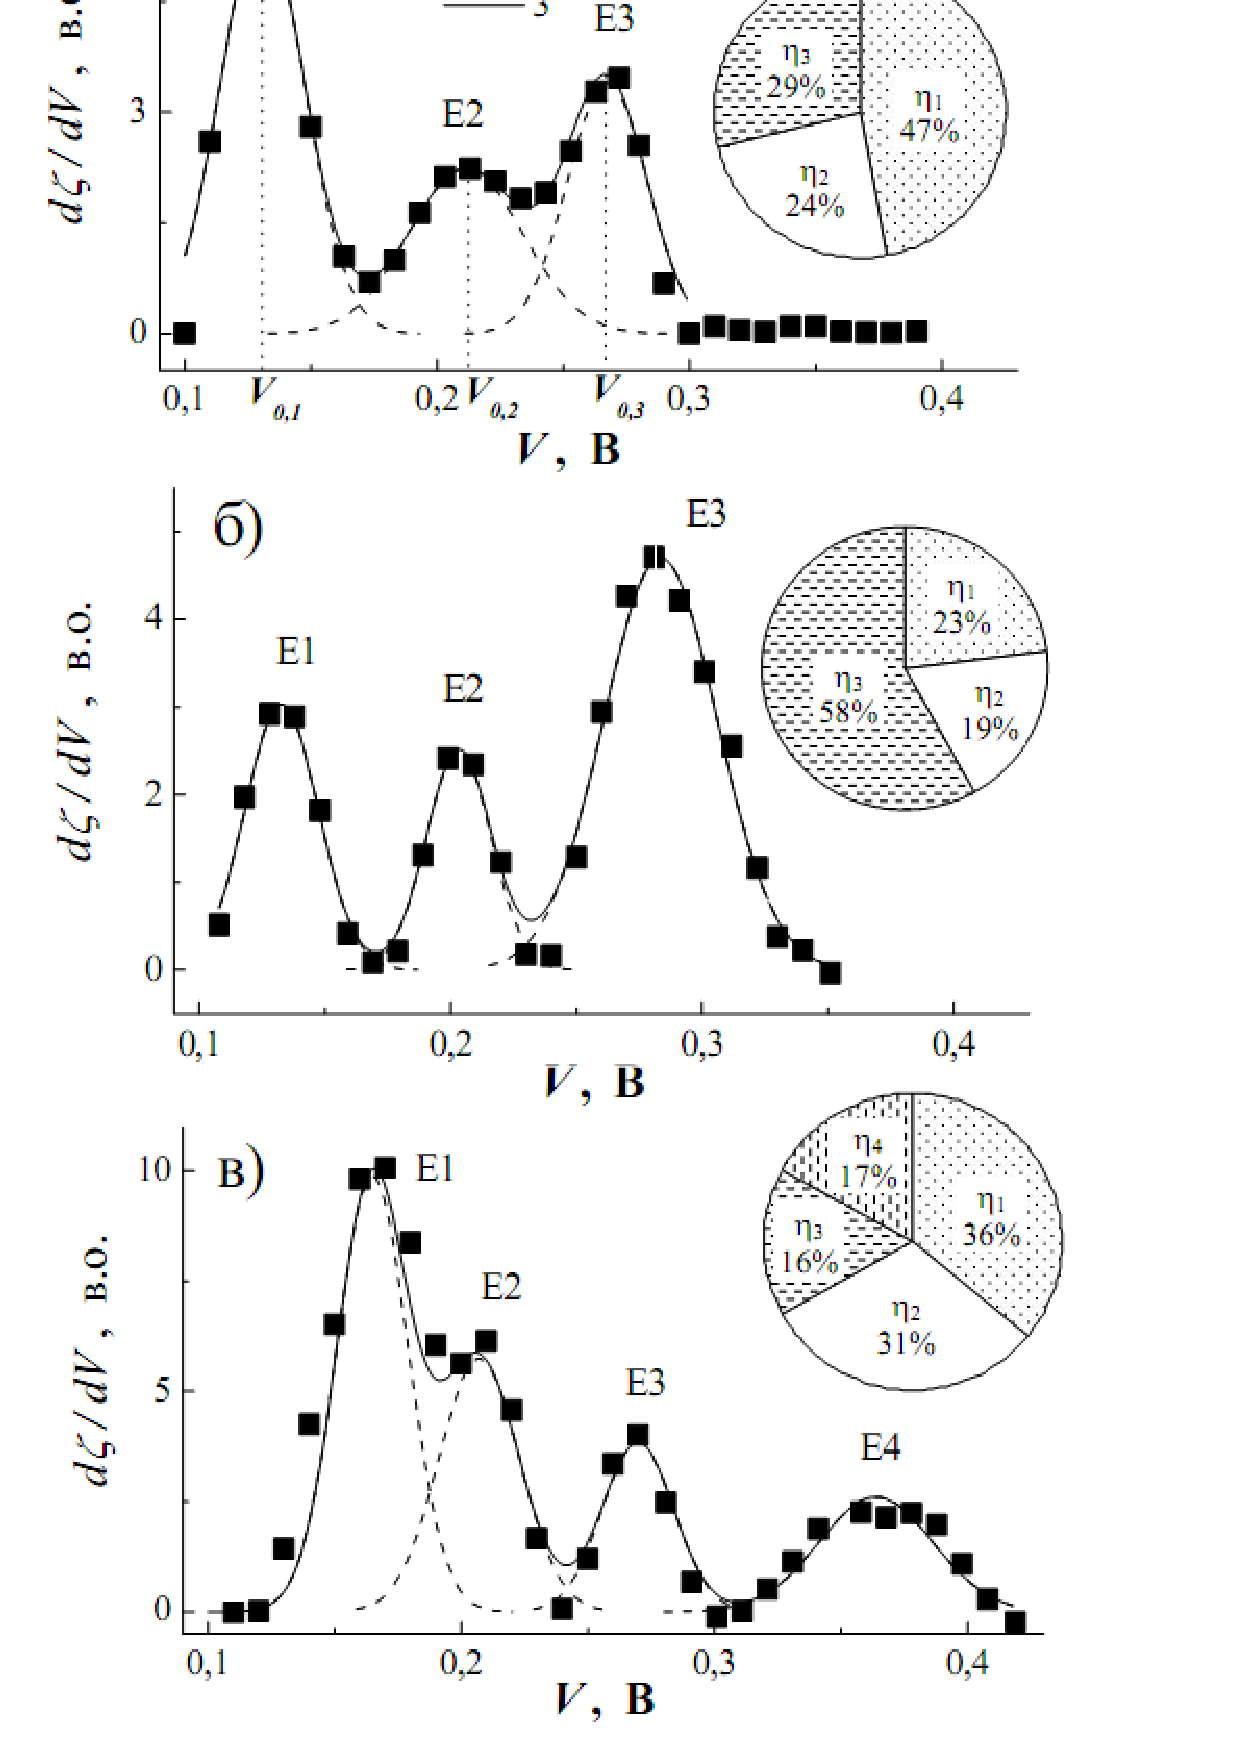
\includegraphics[width=0.65\textwidth]{figBul1}
\caption{\label{figBul1}
Польова залежність похідної диференційного показника нахилу ВАХ у відсутності (а)
та за наявності (б,в) ультразвукового навантаження для кремнієвого сонячного елементу.
1 --- точки, отримані після диференціювання експериментальних ВАХ,
2 --- гаусіани, якими апроксимувалися максимуми,
3 --- сума всіх гаусіан.
Справа біля кривих наведено діаграми відносних внесків $\eta_i$ кожного з максимумів у загальну криву.
Потужність введеного ультразвуку, Вт/см$^2$: $0,1$~(б), $0,25$~(в).
Рисунок взято з роботи \cite{Olikh:FTP2009} з дозволу авторів.
}%
\end{figure}

На рис.~\ref{figBul1} наведено залежності $\partial \zeta/ \partial V = f (V)$, отримані в роботі \cite{Olikh:FTP2009}
для кремнієвих сонячних елементів при відсутності та наявності ультразвукового навантаження (УЗН) структур.
Отримана залежність апроксимована сумою гаусових кривих,
кількість яких визначалась числом максимумів і також проводилась оцінка відносного внеску $\eta_i$ кожного з максимумів у загальну площу
\begin{equation}\label{eqBulEta}
  \eta_i=\frac{S_i}{S_\Sigma}\,,
\end{equation}
де
$S_i$ --- площа під гаусіаною, яка описує $i$--ий максимум,
$S_\Sigma$ --- загальна площа під всією апроксимуючою кривою.
Відповідні дані теж наведено на рисунку.
Величини $\eta_i$ розглядались як показних питомого внеску у загальну рекомбінацію
кожного з глибоких рівнів.
Визначені енергії активації приведені у Таблиці~\ref{tablVAH}.


Одним з недоліків такого підходу є необхідність обчислення других похідних від експериментальних даних.
Тому існує також варіант методу, який передбачає визначення лише перших похідних.
При цьому увага приділяється приведеній швидкості рекомбінації $R_{np}$,
яка, з одного боку, пов'язана з параметрами глибоких рівнів:
\begin{equation}
  R_{np}=\frac{c_n\,c_p\,n_i\,N_t\left[\exp\left(\frac{qV}{2kT}\right)-1\right]}
   {2n_i\sqrt{c_n\,c_p}\exp\left(\frac{qV}{2kT}\right)+n_1\,c_n+p_1\,c_p}\,,
\end{equation}
а з іншого --- може бути визначена з експериментальних даних
\begin{equation}
  R_{np}=\frac{I}{qWA\left[\exp\left(\frac{qV}{2kT}\right)-1\right]}\cdot\frac{q(V_{bi}-V)}{2kT}\,.
\end{equation}
Береться до уваги диференційний коефіцієнт
\begin{equation}
  \zeta_R=\left(\frac{\partial R_{np}}{\partial V}\right)\cdot\frac{2kT}{q}\cdot\frac{1}{R_{np}}\,.
\end{equation}
Напруга, при якій цей коефіцієнт стає мінімальним, дозволяє визначити
енергію активації за формулою (\ref{eqBulEt}) з тією ж систематичною похибкою.
На рис.~\ref{F61} показано приклад подібної залежності.

\begin{figure}[!b]
\center
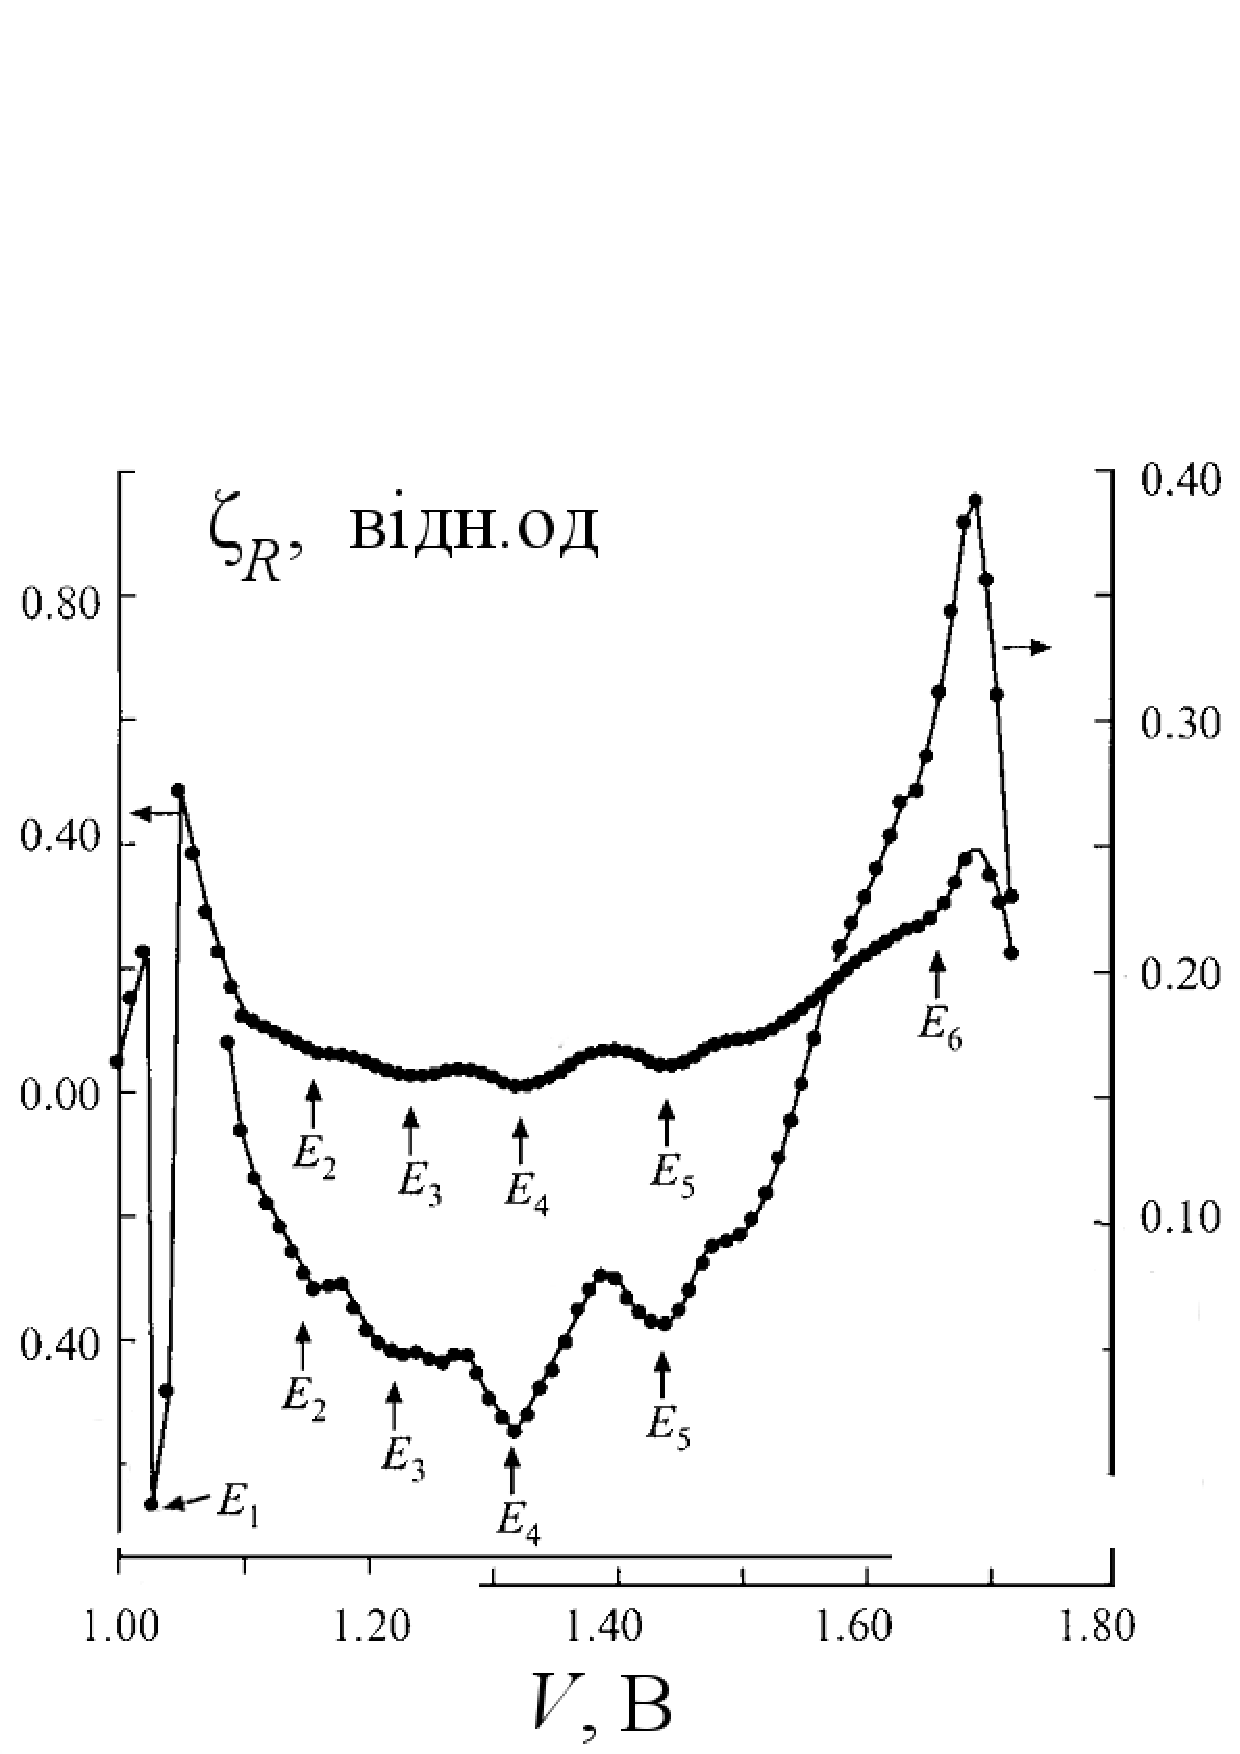
\includegraphics[width=0.65\textwidth]{Fig6_1}
\caption{\label{F61}
Польова залежність диференційного коефіцієнта приведеної швидкості рекомбінації
для GaP світлодіодів (два зразки).
Стрілками вказано мінімуми, розташування
яких дозволили визначити наступні енергії
термічної активації $E_C-E_t$, еВ:
0,61 (рівень $E_1$), 0,54 ($E_2$),
0,46 ($E_3$), 0,41 ($E_4$),
0,37 ($E_5$) та 0,30 ($E_6$).
Рисунок адаптовано з роботи \cite{Bulyar}.
}%
\end{figure}
